\chapter{HASIL DAN PEMBAHASAN}

\section{Pengujian Hyperparameter}

Pengujian \textit{hyperparameter} dilakukan untuk mencari model klasifikasi terbaik, yaitu model yang memenuhi beberapa kriteria berikut:

\begin{enumerate}
    \item Model dapat melakukan klasifikasi dengan baik, ditunjukkan dengan tingkat akurasi klasifikasi terhadap data uji yang tinggi.
    \item Model dapat menyamaratakan dengan baik, ditunjukkan dengan perbedaan yang tidak signifikan antara akurasi klasifikasi data latih dengan akurasi data validasi dan data uji.
    \item Kompleksitas model minimal, sehingga mengurangi beban komputasi dan klasifikasi dapat dilakukan secara \textit{realtime} pada ponsel cerdas.
\end{enumerate}

Variasi \textit{hyperparameter} ditunjukkan pada Tabel~\ref{table:variasi-hyperparameter}. Pengujian dilakukan sebanyak 31 kali dengan variasi \textit{hyperparameter} yang dipilih secara acak. Masing-masing variasi dilatih dalam maksimal 30 \textit{epoch}.

\begin{table}[h!]
    \centering
    \caption{Variasi hyperparameter}
    \begin{tabular}{ |l|c| }
        \hline
        Hyperparameter & Variasi \\

        \hline
        Jumlah lapisan konvolusi & $2 - 4$ \\

        \hline
        Jumlah output konvolusi & $32, 64, 128$ \\

        \hline
        Jumlah lapisan LSTM & $2 - 4$ \\

        \hline
        Jumlah unit LSTM & $32, 64, 128$ \\

        \hline
        Peluang \textit{dropout} & $0,2 - 0,8$ \\

        \hline
        Laju pembelajaran ($\alpha$) & $10^{-4} - 10^{-3}$ \\

        \hline
    \end{tabular}
    \label{table:variasi-hyperparameter}
\end{table}

Hasil pengujian dapat dilihat pada Tabel~\ref{table:hasil-pengujian-hyperparameter}. Perbedaan \textit{hyperparameter} yang digunakan menghasilkan tingkat akurasi klasifikasi yang berbeda. Berdasarkan hasil tersebut, diambil tiga \textit{hyperparameter} dengan akurasi terbaik untuk dibandingkan lebih lanjut, yaitu \textit{hyperparameter} pada model nomor 8, 17 dan 28.

\begin{table}[h!]
    \centering
    \caption{Hasil pengujian \textit{hyperparameter}}
    \pgfplotstabletypeset[
        col sep=comma,
        before row=\hline,every last row/.style={after row=\hline},
        display columns/0/.style={column type=|c|},
        display columns/1/.style={string type, column type=l|},
        display columns/2/.style={string type, column type=l|},
        display columns/3/.style={column type=c|},
        display columns/4/.style={column type=c|,column name=$\alpha$},
        display columns/5/.style={column type=c|,precision=5},
    ]{data/pelatihan/hyperparameter.csv}
    \label{table:hasil-pengujian-hyperparameter}
\end{table}

Model 8 menggunakan empat lapisan konvolusi dan empat lapisan LSTM\@. Keempat lapisan konvolusi menggunakan kernel dengan $64$ output. Lapisan konvolusi pertama menerima input tensor dengan dimensi $100 \times 8$ dan lapisan konvolusi terakhir menghasilkan output tensor dengan ukuran $100 \times 64$. Keempat lapisan LSTM memiliki $32$ unit LSTM\@. Lapisan LSTM pertama menerima input tensor dari output konvolusi dan lapisan LSTM terakhir menghasilkan output tensor dengan ukuran $1 \times 32$. Model ini dilatih dengan peluang \textit{dropout} $0.79$ dan laju pembelajaran $1.46 \times 10^{-4}$.

Proses pelatihan Model 8 dapat dilihat pada Gambar~\ref{gambar:run8-training}. Grafik tersebut menunjukkan peningkatan akurasi klasifikasi dalam proses pelatihan terhadap data latih dan data validasi. Model akhir diambil dari kondisi jaringan saat menghasilkan akurasi terbaik terhadap data validasi, yaitu pada iterasi ke $5069$ dengan akurasi $0.912331$. Pada iterasi yang sama, akurasi terhadap data latih adalah $0.982142$ dan akurasi terhadap data uji adalah $0.91169$.

\begin{figure}[h!]
    \centering
    \includegraphics[width=14cm]{data/pelatihan/run8-accuracy.png}
    \caption{Proses pelatihan pada Model 8}.
    \label{gambar:run8-training}
\end{figure}

\textit{Confusion matrix} Model 8 dapat dilihat pada Gambar~\ref{gambar:run8-confusion-martix}. Pada gambar tersebut dapat dilihat bahwa klasifikasi dilakukan dengan baik pada aktivitas berdiri (96,9\%), duduk (94,9\%) dan lari (96,9\%). Aktivitas jalan memiliki akurasi 87,6\% dan \textit{false negative} yang cukup besar pada naik tangga (8,5\%) dan turun tangga (3,9\%). Aktivitas naik dan turun tangga memiliki klasifikasi terburuk dengan akurasi masing-masing 78,6\% dan 78,4\%, dengan \textit{false negative} tersebar pada seluruh aktivitas lainnya.

\begin{figure}[h!]
    \centering
    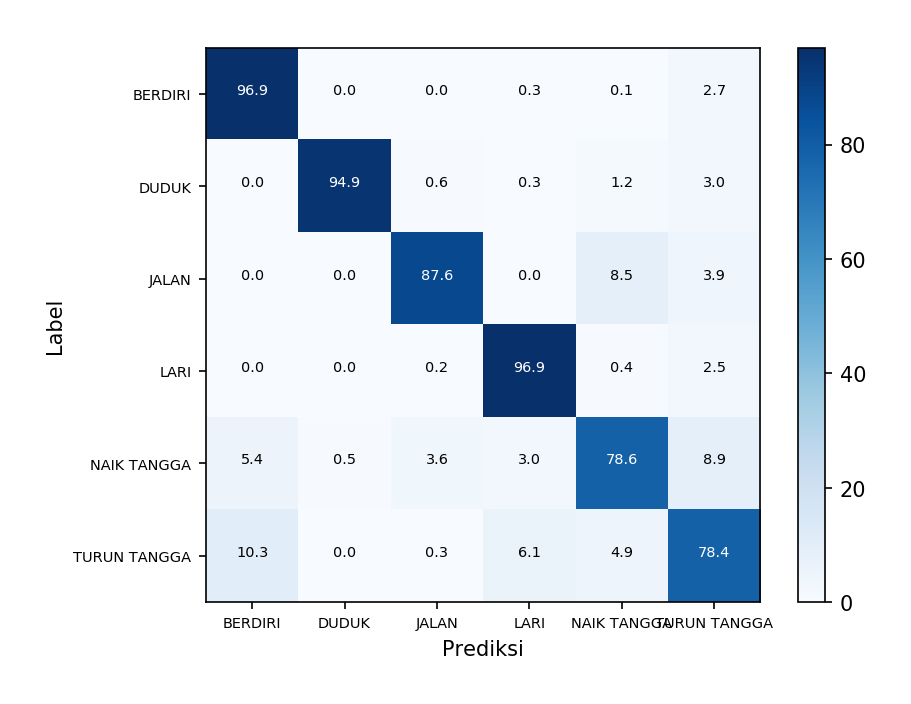
\includegraphics[width=13cm]{gambar/hasil-pembahasan/run8-confusion-matrix.png}
    \caption{\textit{Confusion matrix} pada Model 8}.
    \label{gambar:run8-confusion-martix}
\end{figure}

Model 17 menggunakan tiga lapisan konvolusi dan tiga lapisan LSTM\@. Masing-masing lapisan konvolusi menggunakan kernel dengan $64$ output. Lapisan konvolusi pertama menerima input tensor dengan dimensi $100 \times 8$ dan lapisan konvolusi terakhir menghasilkan output tensor dengan ukuran $100 \times 64$. Masing-masing lapisan LSTM memiliki $64$ unit LSTM\@. Lapisan LSTM pertama menerima input tensor dari output konvolusi dan lapisan LSTM terakhir menghasilkan output tensor dengan ukuran $1 \times 64$. Model ini dilatih dengan peluang \textit{dropout} $0.59$ dan laju pembelajaran $2.81 \times 10^{-4}$.

Proses pelatihan Model 17 dapat dilihat pada Gambar~\ref{gambar:run17-training}. Model akhir diambil dari kondisi jaringan saat menghasilkan akurasi terbaik terhadap data validasi, yaitu pada iterasi ke $4394$ dengan akurasi $0.929793$. Pada iterasi yang sama, akurasi terhadap data latih adalah $1.0$ dan akurasi terhadap data uji  $0.93652$.

\begin{figure}[h!]
    \centering
    \includegraphics[width=14cm]{data/pelatihan/run17-accuracy.png}
    \caption{Proses pelatihan pada Model 17}.
    \label{gambar:run17-training}
\end{figure}

\textit{Confusion matrix} Model 17 dapat dilihat pada Gambar~\ref{gambar:run17-confusion-martix}. Pada gambar tersebut dapat dilihat bahwa klasifikasi dilakukan dengan baik pada aktivitas berdiri (97,2\%), duduk (93,4\%) dan jalan (96,1\%). Aktivitas lari memiliki akurasi 85,5\% dan \textit{false negative} yang cukup besar pada jalan (8,6\%) dan turun tangga (5,7\%). Aktivitas naik dan turun tangga memiliki akurasi masing-masing 81,2\% dan 82,4\%, dengan \textit{false negative} tersebar pada seluruh aktivitas lainnya.

\begin{figure}[h!]
    \centering
    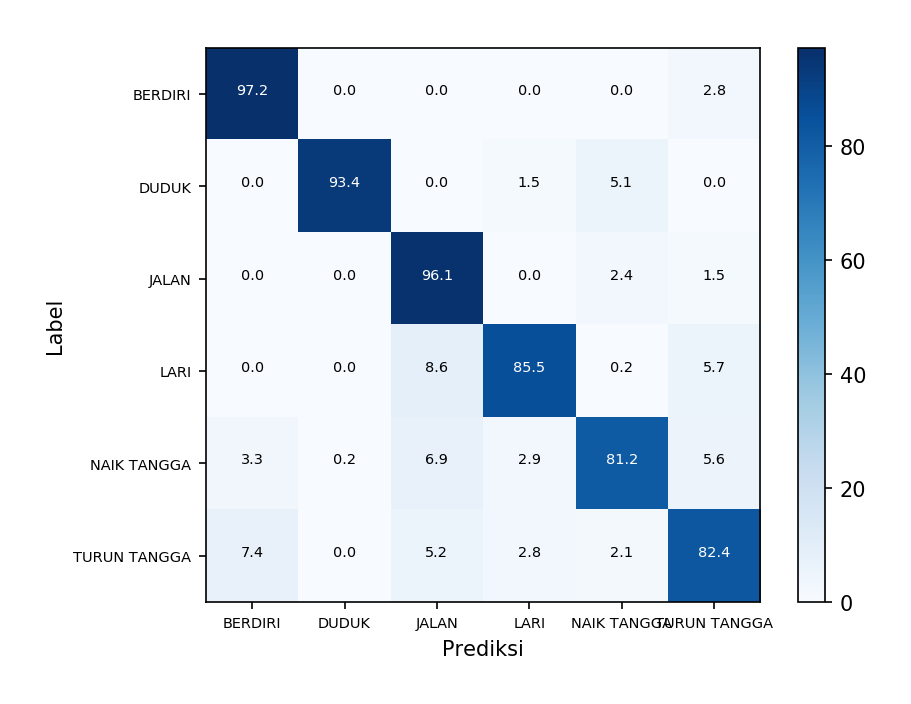
\includegraphics[width=13cm]{gambar/hasil-pembahasan/run17-confusion-matrix.png}
    \caption{\textit{Confusion matrix} pada Model 17}.
    \label{gambar:run17-confusion-martix}
\end{figure}

Model 28 menggunakan empat lapisan konvolusi dan tiga lapisan LSTM\@. Masing-masing lapisan konvolusi menggunakan kernel dengan $64$ output. Lapisan konvolusi pertama menerima input tensor dengan dimensi $100 \times 8$ dan lapisan konvolusi terakhir menghasilkan output tensor dengan ukuran $100 \times 64$. Masing-masing lapisan LSTM memiliki $32$ unit LSTM\@. Lapisan LSTM pertama menerima input tensor dari output konvolusi dan lapisan LSTM terakhir menghasilkan output tensor dengan ukuran $1 \times 32$. Model ini dilatih dengan peluang \textit{dropout} $0.76$ dan laju pembelajaran $4.14 \times 10^{-4}$.

Proses pelatihan Model 28 dapat dilihat pada Gambar~\ref{gambar:run34-training}. Model akhir diambil dari kondisi jaringan saat menghasilkan akurasi terbaik terhadap data validasi, yaitu pada iterasi ke $4901$ dengan akurasi $0.896472$. Pada iterasi yang sama, akurasi terhadap data latih adalah $0.9375$ dan akurasi terhadap data uji  $0.93153$.

\begin{figure}[h!]
    \centering
    \includegraphics[width=14cm]{data/pelatihan/run34-accuracy.png}
    \caption{Proses pelatihan pada Model 28}.
    \label{gambar:run34-training}
\end{figure}

\textit{Confusion matrix} Model 28 dapat dilihat pada Gambar~\ref{gambar:run34-confusion-martix}. Pada gambar tersebut dapat dilihat bahwa klasifikasi dilakukan dengan baik pada aktivitas berdiri (99,4\%), jalan (98,4\%) dan lari (94,6\%). Aktivitas duduk memiliki akurasi 77,4\% dan \textit{false negative} yang besar pada jalan (16,6\%). Aktivitas naik dan turun tangga memiliki akurasi masing-masing 62,2\% dan 58,3\%, dengan \textit{false negative} tersebar pada seluruh aktivitas lainnya.

\begin{figure}[h!]
    \centering
    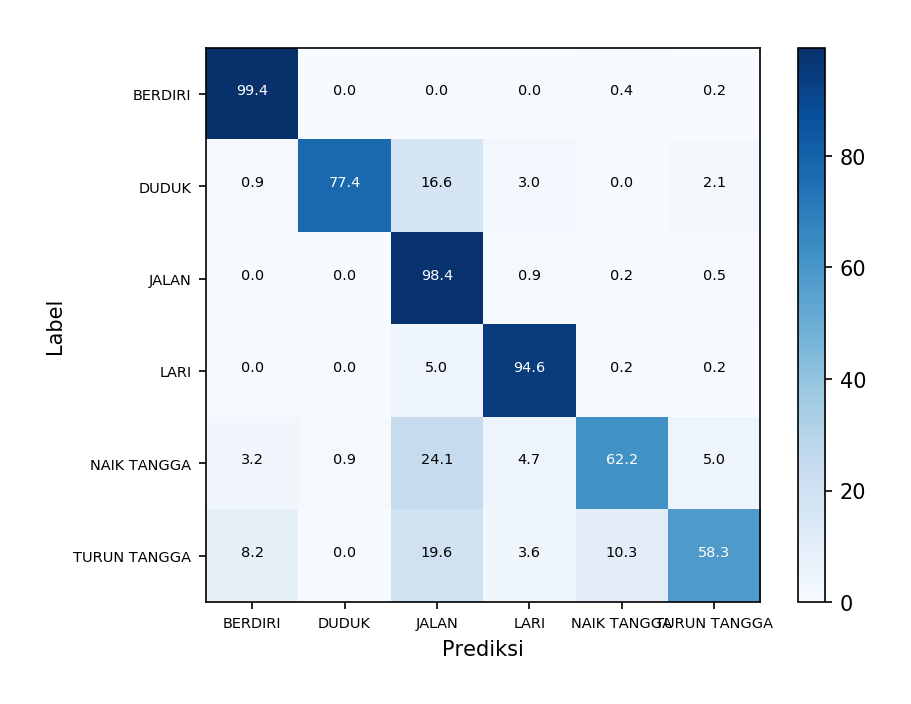
\includegraphics[width=13cm]{gambar/hasil-pembahasan/run34-confusion-matrix.png}
    \caption{\textit{Confusion matrix} pada Model 28}.
    \label{gambar:run34-confusion-martix}
\end{figure}

Hasil pengujian Model 8, 17 dan 28 dibandingkan dalam Tabel~\ref{table:perbandingan-model-klasifikasi}. Ketiga model tersebut memiliki kelebihan dan kekurangannya masing-masing. Model nomor 8 memperoleh akurasi tertinggi pada aktivitas duduk dan lari, namun memperoleh akurasi terendah pada aktivitas berdiri, jalan dan rata-rata akurasi. Model nomor 17 memperoleh akurasi tertinggi pada aktivitas naik tangga, turun tangga dan rata-rata akurasi, namun memperoleh akurasi terendah pada aktivitas duduk dan lari. Selain itu model nomor 17 juga memiliki arsitektur yang paling sederhana diantara model lainnya. Model nomor 28 memperoleh akurasi terbaik pada aktivitas berdiri dan jalan, namun memperoleh akurasi terburuk pada aktivitas naik dan turun tangga. Melihat grafik pada Gambar~\ref{gambar:run8-training},~\ref{gambar:run17-training}, dan~\ref{gambar:run34-training}, diketahui bahwa ketiga model memiliki penyamarataan yang setara baiknya.

\begin{table}[h!]
    \centering
    \caption{Perbandingan model klasifikasi}
    \begin{threeparttable}
        \begin{tabular}{ |c|c|c|c|c|c|c|c| }
            \hline
            No & B & D & J & L & N & T & Akurasi \\

            \hline
            8 & \cellcolor{red!10} 96,9\% & \cellcolor{teal!20}94,9\% & \cellcolor{red!10} 87,6\% & \cellcolor{teal!20} 96,9\% & 78,6\% & 78,4\% & \cellcolor{red!10} 91,17\% \\

            \hline
            17 & 97,2\% & \cellcolor{red!10} 93,4\% & 96,1\% & \cellcolor{red!10} 85,5\% & \cellcolor{teal!20} 81,2\% & \cellcolor{teal!20} 82,2\% & \cellcolor{teal!20} 93,65\% \\

            \hline
            28 & \cellcolor{teal!20} 99,4\% & 77,4\% & \cellcolor{teal!20} 98,4\% & 94,6\% & \cellcolor{red!10} 62,2\% & \cellcolor{red!10} 58,3\% & 93,15\% \\

            \hline
        \end{tabular}
        \begin{tablenotes}\footnotesize
            \item  B: Berdiri, D: Duduk, J: Berjalan, L: Berlari, N: Naik Tangga, T: Turun Tangga 
        \end{tablenotes}    
    \end{threeparttable}
    \label{table:perbandingan-model-klasifikasi}
\end{table}

Berdasarkan pertimbangan kriteria akurasi, penyamarataan dan kompleksitas model, maka model nomor 17 dipilih sebagai model terbaik. Model ini kemudian diimplementasikan pada ponsel cerdas untuk pengujian akurasi klasifikasi online dan pengujian waktu komputasi.

\section{Hasil Pengujian Klasifikasi \textit{Online}}

Pengujian klasifikasi \textit{online} dilakukan untuk mengetahui kemampuan klasifikasi model secara \textit{realtime} pada ponsel cerdas. Pengujian ini dilakukan oleh 6 partisipan dengan jenis kelamin dan usia yang dijelaskan pada Tabel~\ref{table:partisipan}.

\begin{table}[h!]
    \centering
    \caption{Partisipan pengujian}
    \begin{tabular}{ |c|l|c| }
        \hline
        Partisipan & Jenis Kelamin & Usia \\

        \hline
        1 & Perempuan & 21 \\

        \hline
        2 & Laki-laki & 22 \\

        \hline
        3 & Laki-laki & 21 \\

        \hline
        4 & Laki-laki & 21 \\

        \hline
        5 & Perempuan & 21 \\

        \hline
        6 & Perempuan & 21 \\

        \hline
    \end{tabular}
    \label{table:partisipan}
\end{table}

Pada proses pengujian, partisipan melakukan aktivitas duduk, berdiri, berjalan, berlari, menaiki tangga dan menuruni tangga dengan menempatkan ponsel cerdas di saku celana sebelah kanan. Masing-masing aktivitas dilakukan selama satu menit, menghasilkan 1632 sampel dari seluruh aktivitas.

\begin{table}[h!]
    \centering
    \caption{Hasil klasifikasi seluruh aktivitas}
    \begin{threeparttable}
        \pgfplotstabletypeset[
            col sep=comma,
            before row=\hline,every last row/.style={after row=\hline},
            display columns/0/.style={string type, column type=|c|},
            display columns/1/.style={column name=D (\%), column type=c|},
            display columns/2/.style={column name=B (\%), column type=c|},
            display columns/3/.style={column name=J (\%), column type=c|},
            display columns/4/.style={column name=L (\%), column type=c|},
            display columns/5/.style={column name=N (\%), column type=c|},
            display columns/6/.style={column name=T (\%), column type=c|},
            display columns/7/.style={column name=Akurasi (\%), column type=c|,precision=3},
        ]{data/prediksi/partisipan.data}
        \begin{tablenotes}\footnotesize
            \item  D: Duduk, B: Berdiri, J: Berjalan, L: Berlari, N: Naik Tangga, T: Turun Tangga 
        \end{tablenotes}
    \end{threeparttable}
    \label{table:hasil-klasifikasi-online}
\end{table}

Hasil pengujian klasifikasi online dapat dilihat pada Tabel~\ref{table:hasil-klasifikasi-online}. Seluruh partisipan mendapatkan akurasi 100\% pada aktivitas berdiri dan berlari. Aktivitas duduk memperoleh akurasi 100\% pada lima partisipan, sedangkan satu partisipan lainnya memperoleh akurasi 98.15\% sehingga rata-rata akurasi aktivitas duduk adalah 99.63\%.

Aktivitas berjalan memperoleh akurasi yang baik pada partisipan 2, 3, 4, dan 6, namun memperoleh akurasi yang kurang baik pada partisipan 1 (78,85\%) dan partisipan 2 (81,48\%). Rata-rata akurasi aktivitas berjalan adalah 88\%. Aktivitas menaiki tangga dan menuruni tangga memperoleh tingkat akurasi yang kurang baik. Rata-rata akurasi menaiki tangga adalah 69,1\% dan rata-rata akurasi menuruni tangga adalah 81,82\%. Dari seluruh partisipan, diperoleh rata-rata akurasi seluruh aktivitas sebesar 89,757\%.

\begin{figure}[h!]
    \centering
    \includegraphics[width=13cm]{data/prediksi/confusion-matrix.png}
    \caption{\textit{Confusion matrix} pengujian \textit{online}}.
    \label{gambar:online-confusion-martix}
\end{figure}

Klasifikasi masing-masing aktivitas dapat dilihat lebih jelas melalui \textit{confusion matrix} pada Gambar~\ref{gambar:online-confusion-martix}. Dari \textit{confusion matrix} dapat dilihat beberapa kelasahan klasifikasi yang terjadi, yaitu:

\begin{itemize}
    \item Sebesar 12\% aktivitas berjalan diklasifikasikan sebagai naik tangga (8,2\%) dan turun tangga (3,8\%).
    \item Sebesar 29,9\% aktivitas naik tangga diklasifikasikan sebagai jalan (25,8\%) dan turun tangga (4,1\%).
    \item Sebesar 18,2\% aktivitas turun tangga diklasifikasikan sebagai jalan (12,5\%) dan naik tangga (5,7\%).
\end{itemize}

Hasil pengujian klasifikasi \textit{online} ini konsisten dengan pengujian \textit{offline}. Aktivitas duduk, berdiri, jalan dan lari dapat diklasifikasi dengan akurasi yang cukup tinggi, sedangkan akurasi pada aktivitas menaiki tangga dan menuruni tangga tidak terlalu baik.

Aktivitas duduk, berdiri, jalan dan lari dapat diklasifikasikan dengan baik karena perbedaan pola yang signifikan pada data-data sensornya, sedangkan aktivitas menaiki tangga dan menuruni tangga memperoleh akurasi yang kurang baik karena pola data sensor yang cukup mirip. Kedua aktivitas tersebut juga memiliki kemiripan dengan aktivitas jalan, sehingga banyak terjadi kesalahan dalam mengklasifikasikan aktivitas menaiki tangga dan menuruni tangga menjadi jalan. Perbandingan pola tersebut dapat dilihat pada Gambar~\ref{gambar:plot-sensor} yang menunjukkan sampel data sensor dari masing-masing aktivitas.

\begin{figure}[h!]
    \begin{subfigure}{0.5\textwidth}
        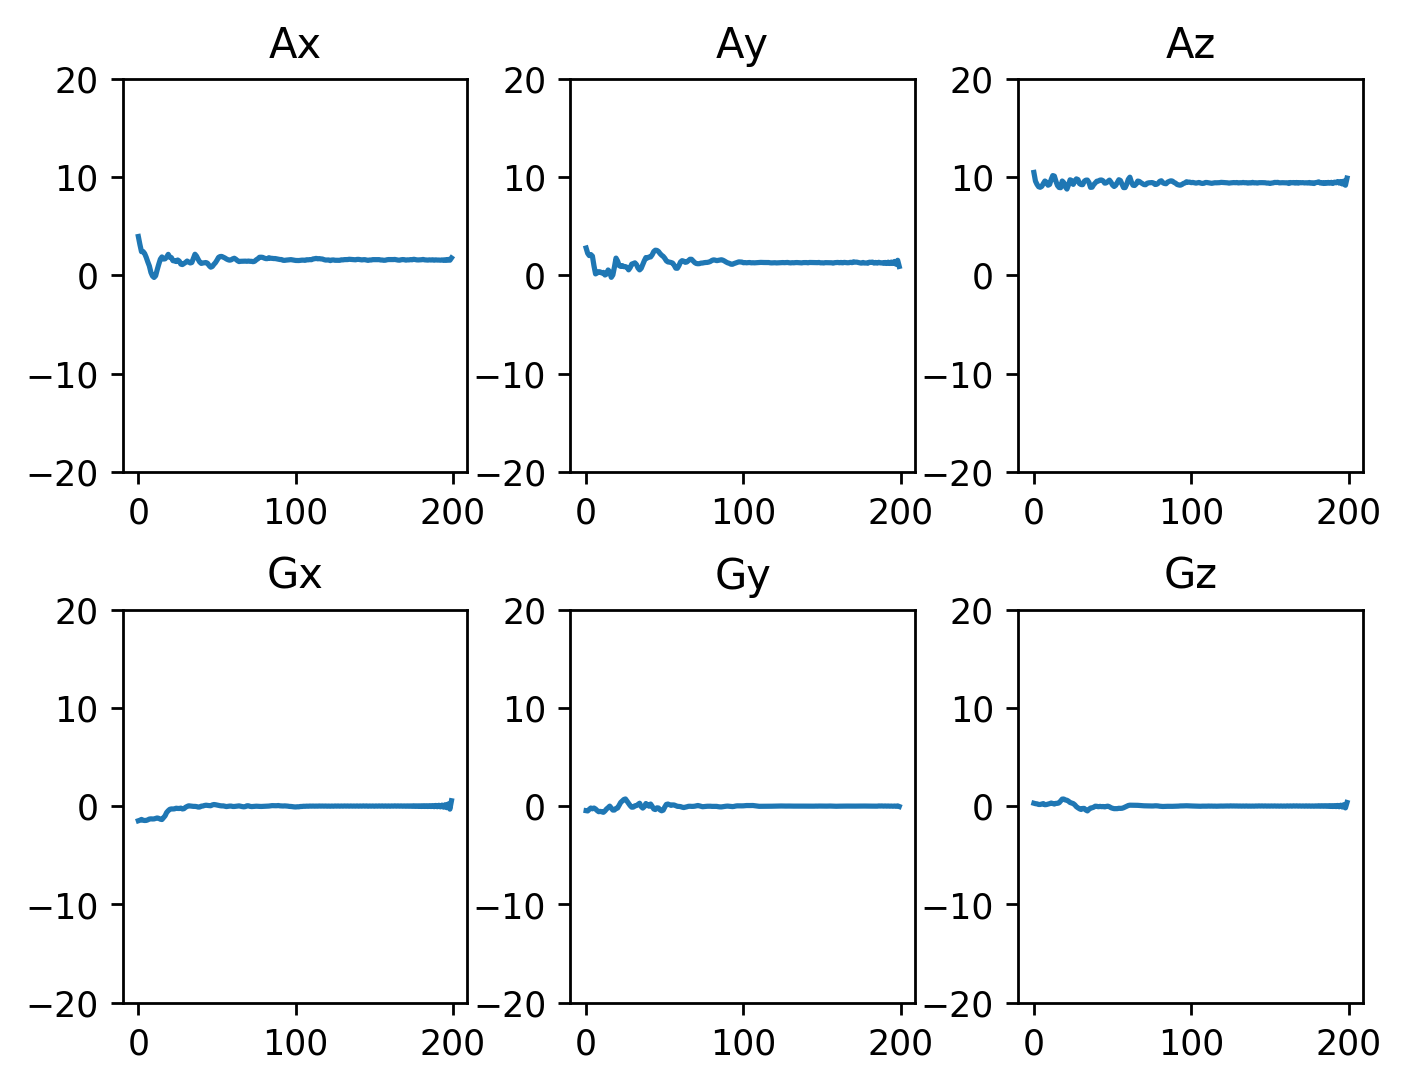
\includegraphics[width=7.2cm]{data/plot-sensor/duduk.png}
        \caption{Duduk}
        \label{gambar:plot-sensor-duduk}
    \end{subfigure}
    \begin{subfigure}{0.5\textwidth}
        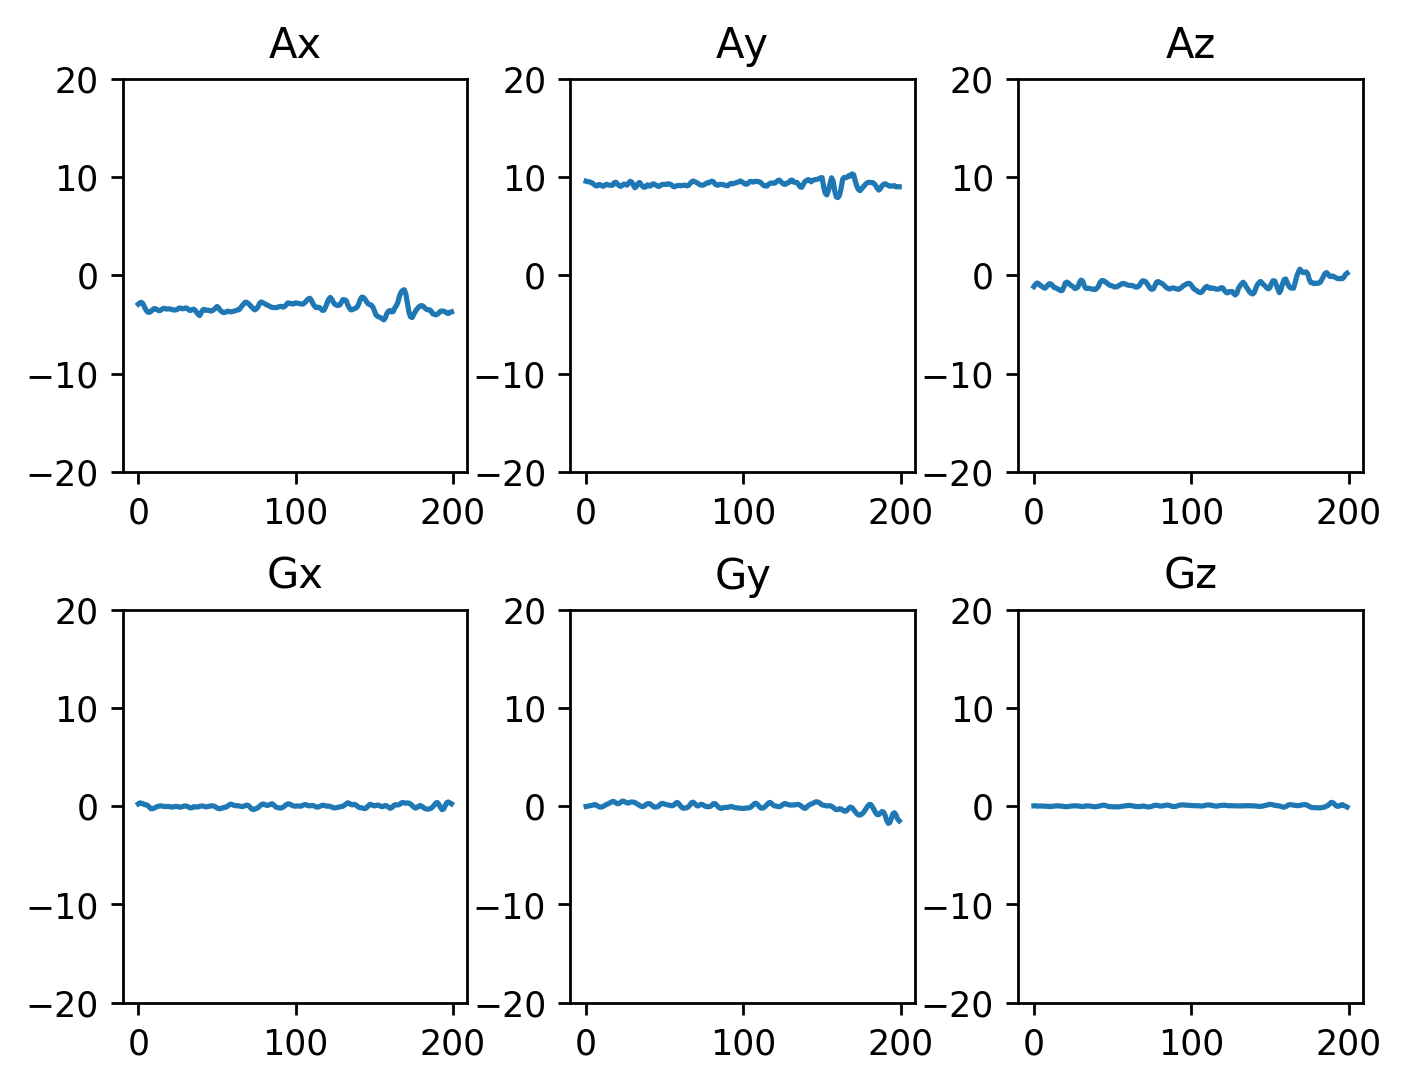
\includegraphics[width=7.2cm]{data/plot-sensor/berdiri.png}
        \caption{Berdiri}
        \label{gambar:plot-sensor-berdiri}
    \end{subfigure}
    \begin{subfigure}{0.5\textwidth}
        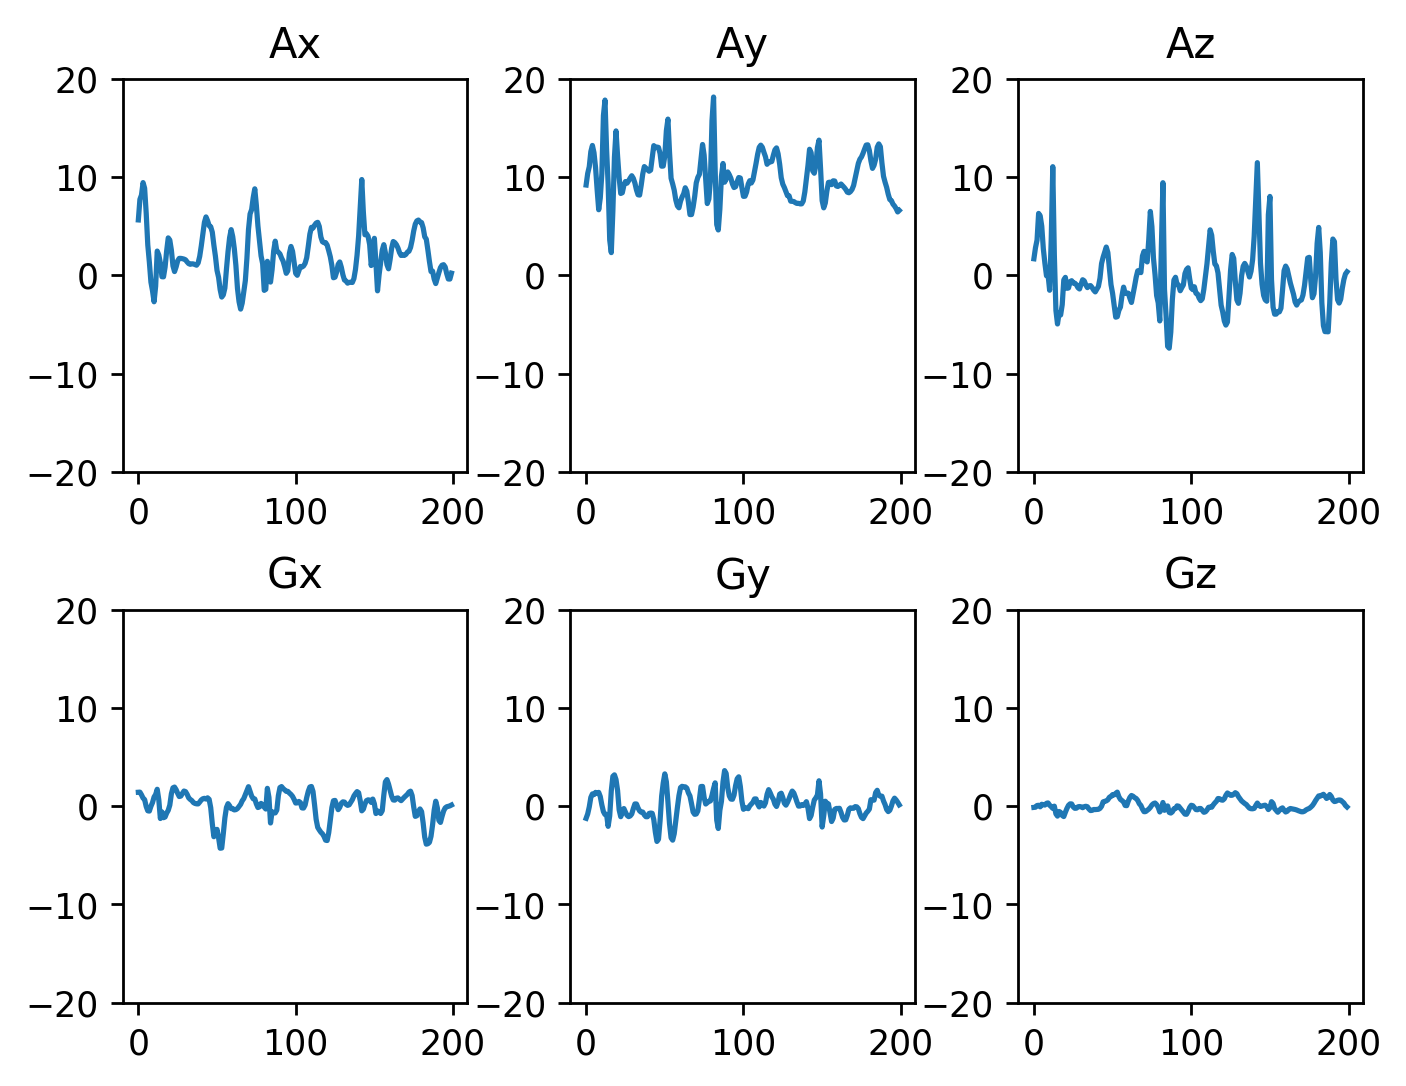
\includegraphics[width=7.2cm]{data/plot-sensor/berjalan.png}
        \caption{Berjalan}
        \label{gambar:plot-sensor-berjalan}
    \end{subfigure}
    \begin{subfigure}{0.5\textwidth}
        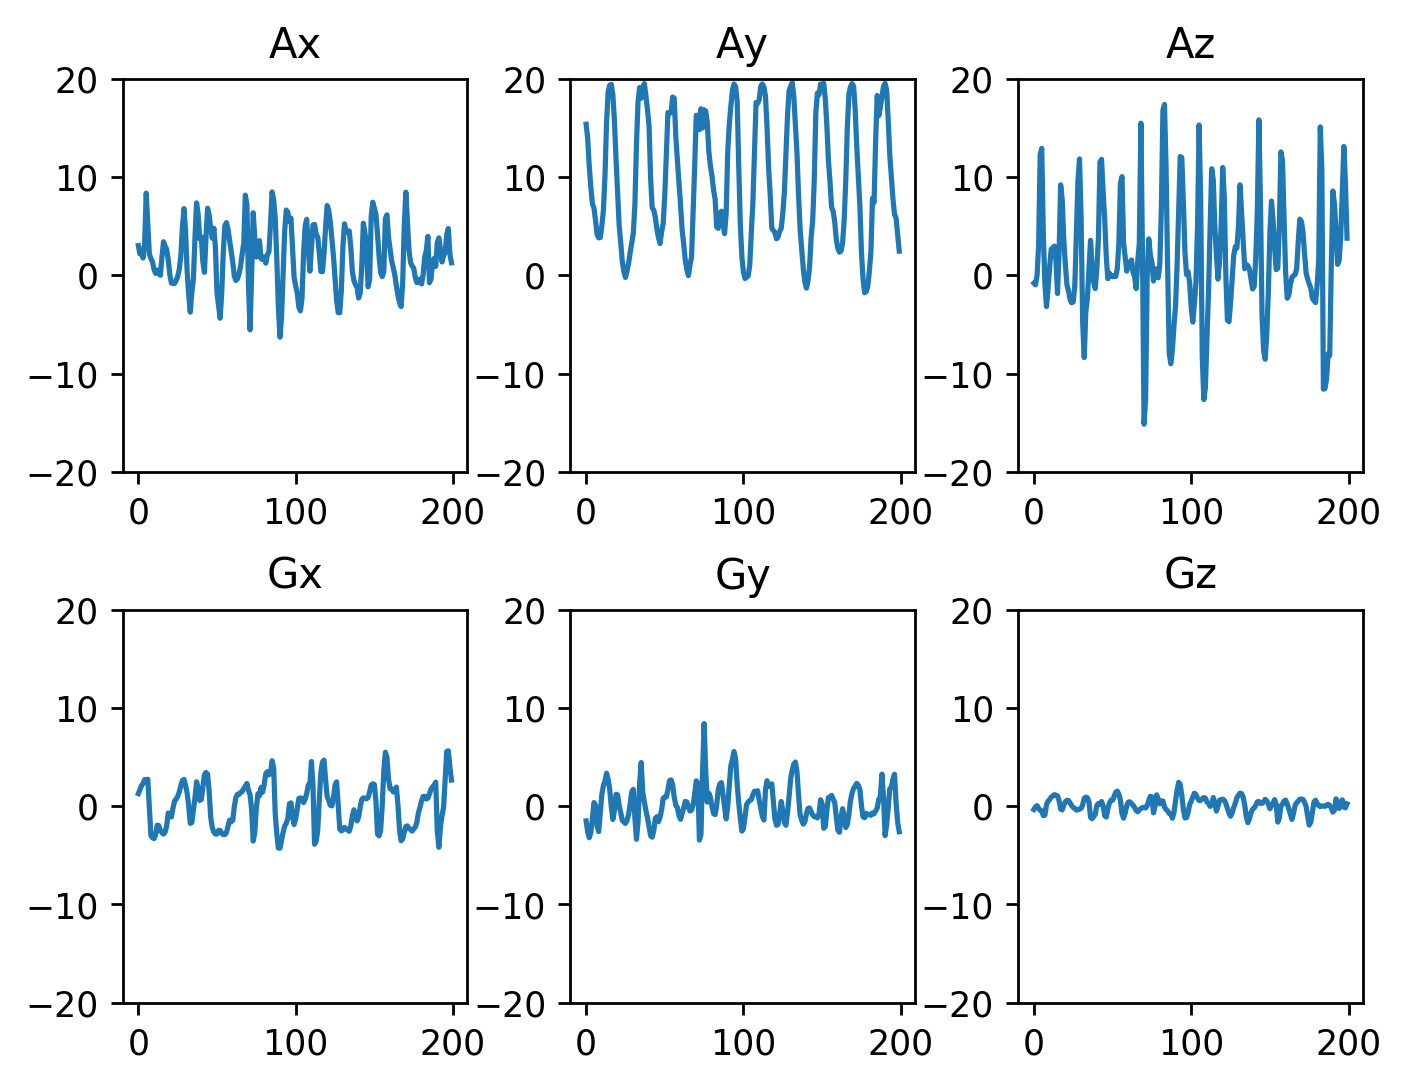
\includegraphics[width=7.2cm]{data/plot-sensor/berlari.png}
        \caption{Berlari}
        \label{gambar:plot-sensor-berlari}
    \end{subfigure}
    \begin{subfigure}{0.5\textwidth}
        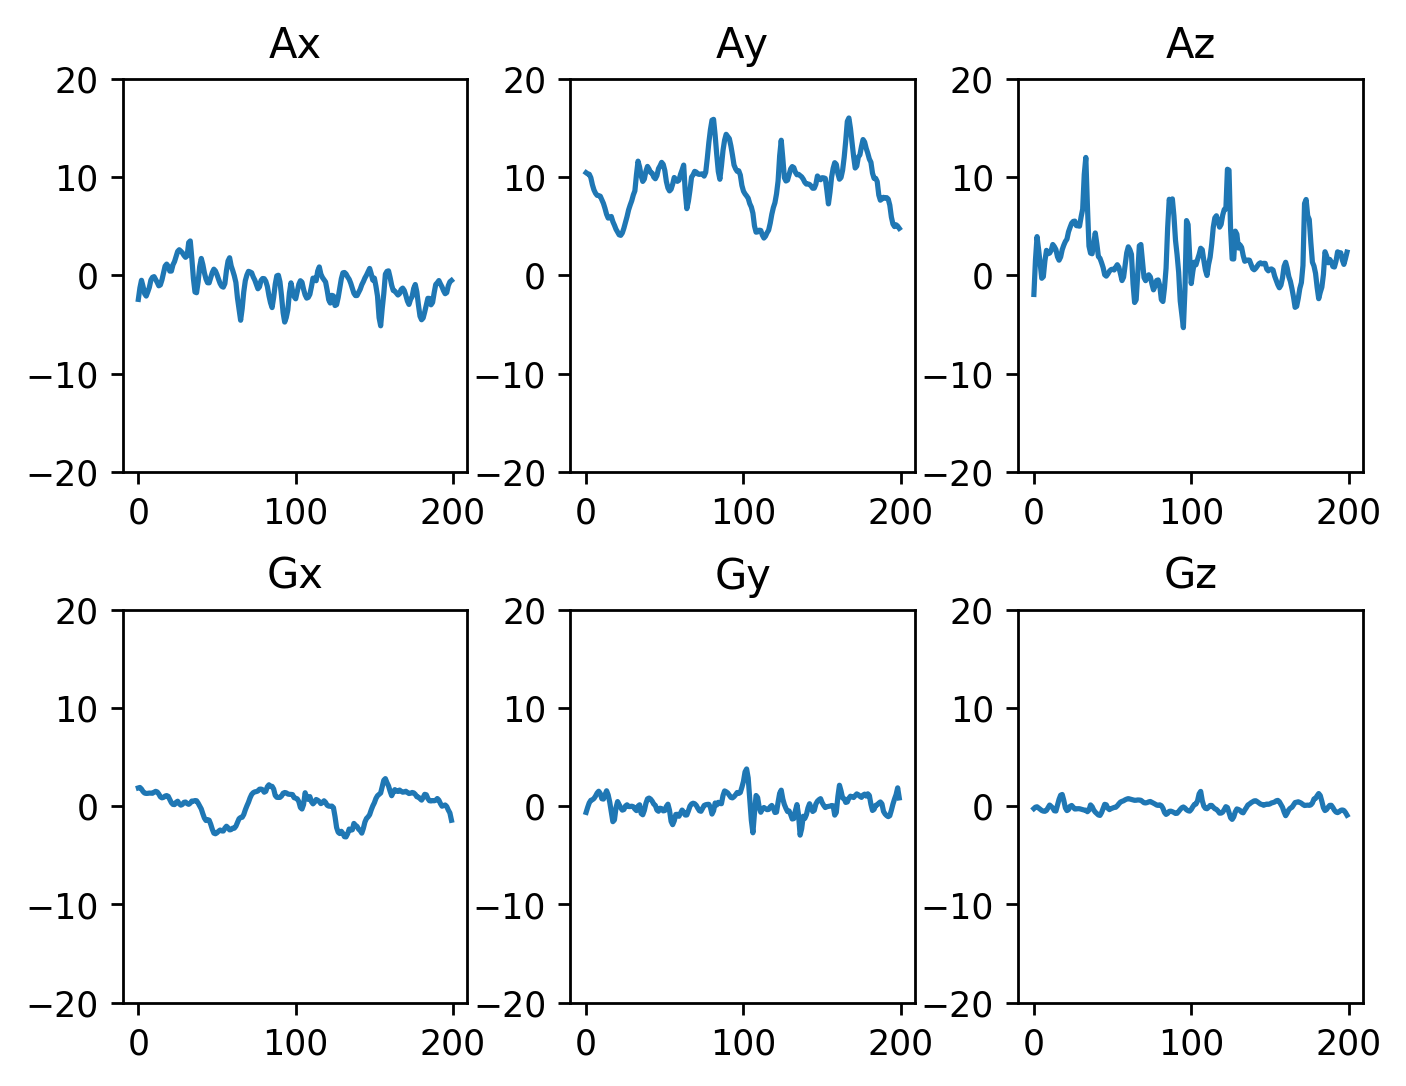
\includegraphics[width=7.2cm]{data/plot-sensor/naik-tangga.png}
        \caption{Menaiki tangga}
        \label{gambar:plot-sensor-naik-tangga}
    \end{subfigure}
    \begin{subfigure}{0.5\textwidth}
        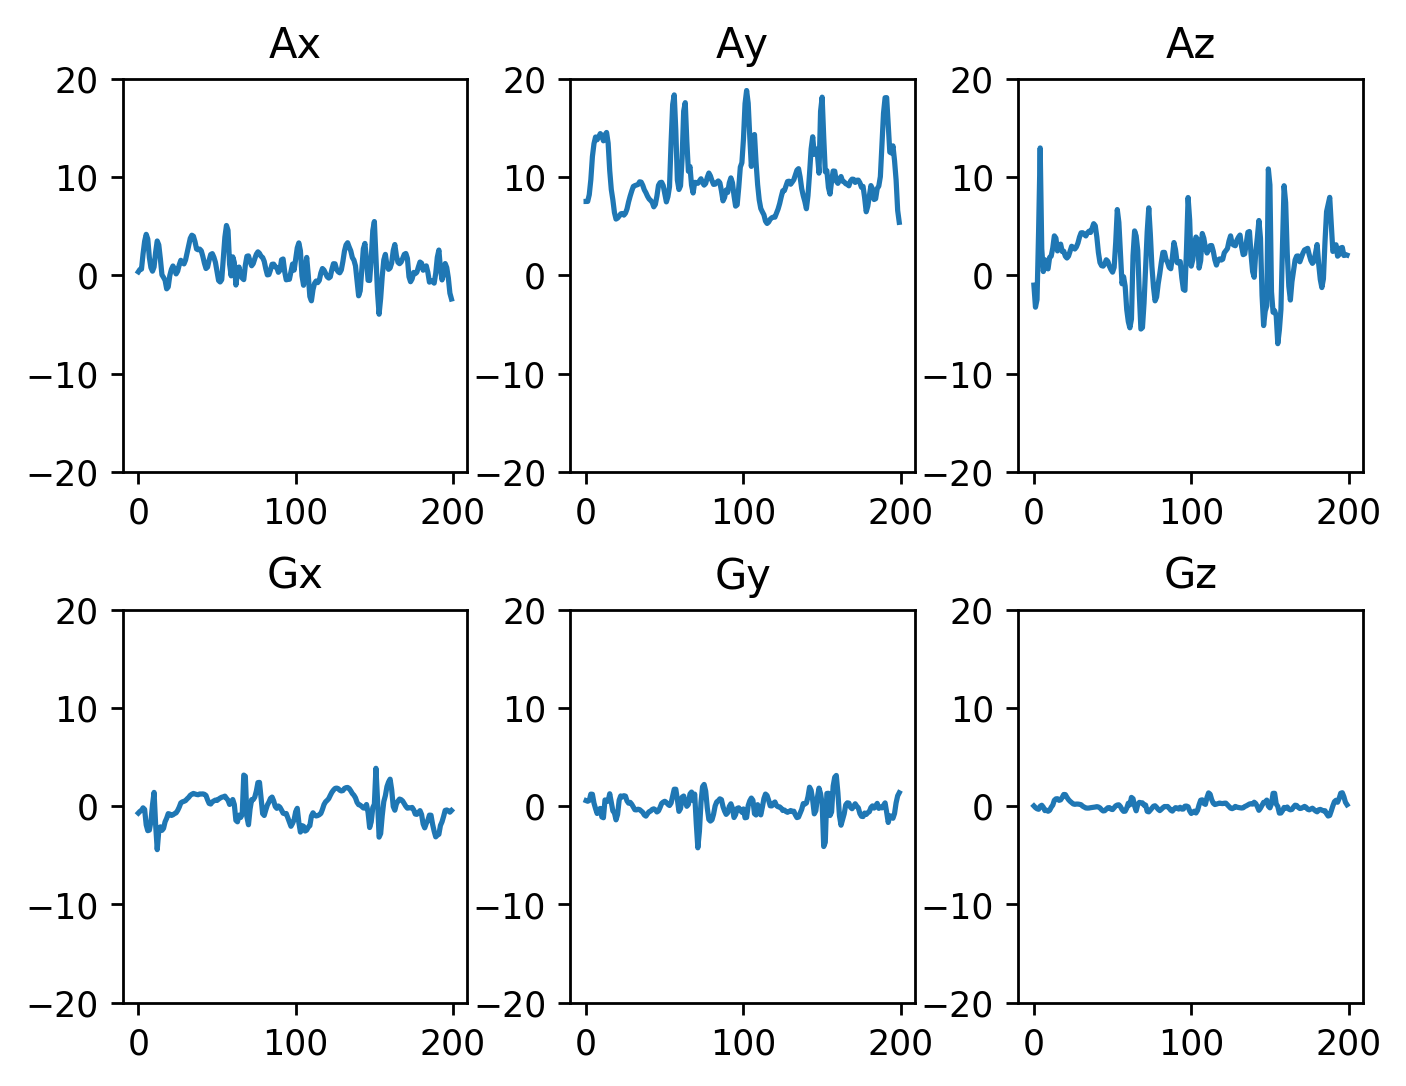
\includegraphics[width=7.2cm]{data/plot-sensor/turun-tangga.png}
        \caption{Menuruni tangga}
        \label{gambar:plot-sensor-turun-tangga}
    \end{subfigure}

    \caption{Perbandingan sinyal sensor dari setiap aktivitas}
    \label{gambar:plot-sensor}
\end{figure}

\section{Hasil Pengujian Kecepatan Klasifikasi pada Ponsel Cerdas}

Pengujian kecepatan klasifikasi pada ponsel cerdas dilakukan untuk mengetahui waktu komputasi yang dibutuhkan model dalam mengklasifikasikan aktivitas pada perangkat dengan kemampuan komputasi yang terbatas. Semakin cepat komputasi dilakukan, maka model dinilai semakin baik digunakan untuk klasifikasi secara \textit{realtime}.

Klasifikasi dilakukan pada tiga ponsel cerdas yang berbeda, yaitu Xiaomi Mi4c dan LG G5 SE, dan vivo V5. Spesifikasi kedua ponsel cerdas tersebut dapat dilihat pada Tabel~\ref{table:spesifikasi-ponsel-cerdas}.

\begin{table}[h!]
    \centering
    \caption{Spesifikasi ponsel cerdas untuk pengujian}
    \begin{tabular}{ |l|l|c|c| }
        \hline
        Ponsel & CPU & Memori & Total Prediksi \\

        \hline
        Xiaomi Mi4c & Snapdragon 805 & 2 GB & 887 \\

        \hline
        LG G5 SE & Snapdragon 652 & 3 GB & 413 \\

        \hline
        vivo V5 & Mediatek MT6750 & 4 GB & 332 \\

        \hline
    \end{tabular}
    \label{table:spesifikasi-ponsel-cerdas}
\end{table}

Pengujian dilakukan dengan mencatat waktu komputasi yang diperlukan pada setiap iterasi klasifikasi. Perhitungan waktu dimulai saat jendela data sensor siap digunakan sampai diperoleh prediksi aktivitas. Kecepatan klasifikasi pada ponsel Xiaomi Mi4c diukur oleh tiga partisipan dengan total 887 sampel, kecepatan pada LG G5 SE diukur oleh dua partisipan dengan total 413 sampel, sedangkan kecepatan pada vivo V5 diukur oleh satu partisipan dengan total 332 sampel. Nilai minimum, maksimum, median dan rata-rata diambil dari data yang telah dikumpulkan.

Hasil pengujian dapat dilihat pada Gambar~\ref{gambar:hasil-kecepatan}. Dari 887 klasifikasi yang dilakukan pada ponsel Xiaomi Mi4c, diperoleh waktu komputasi minimal 78 ms, median 148 ms, maksimal 280 ms dan rata-rata 147 ms. Pada ponsel LG G5 SE, dari 413 klasifikasi yang dilakukan, diperoleh waktu komputasi minimal 83 ms, median 176 ms, maksimal 271 ms dan rata-rata 167 ms. Dari 332 klasifikasi yang dilakukan pada ponsel vivo V5, diperoleh waktu komputasi minimal 161 ms, median 229 ms, maksimal 389 ms dan rata-rata 255 ms.

\begin{figure}[h!]
    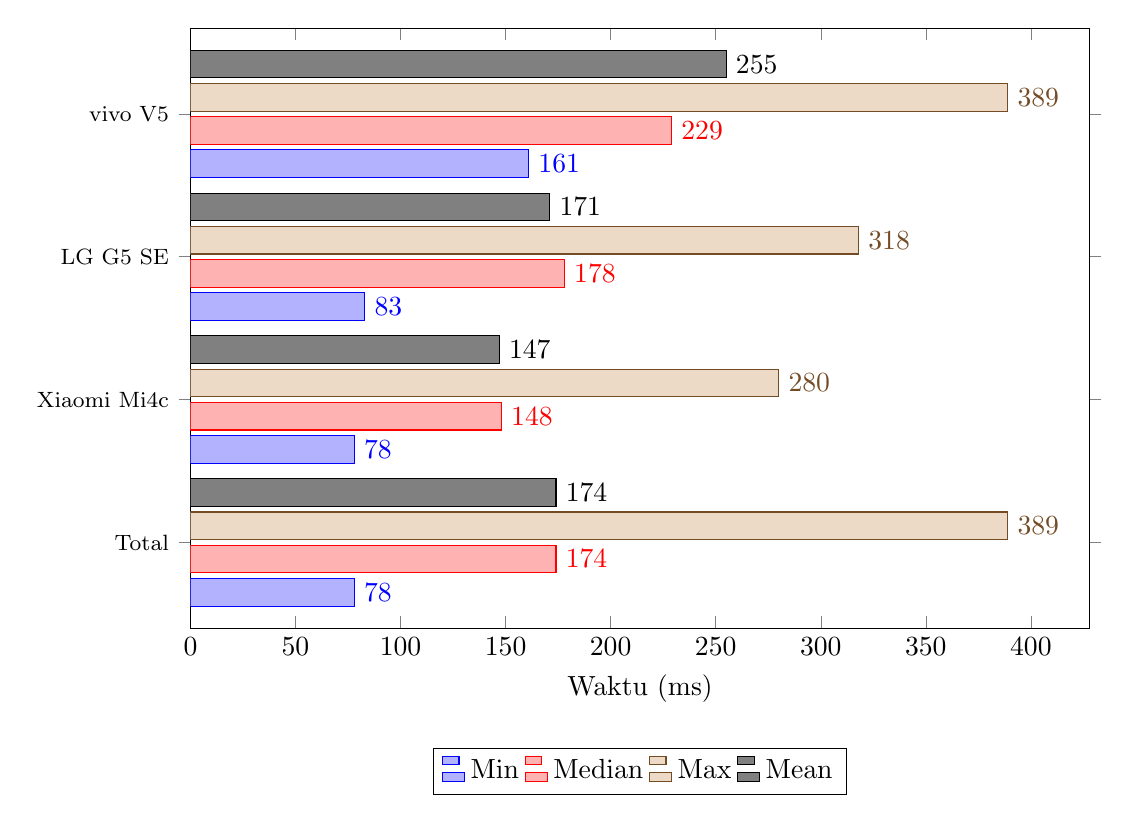
\begin{tikzpicture}
    \begin{axis}[
        xbar, xmin=0,
        y tick label style={font=\footnotesize},
        width=13cm, height=9.2cm, enlarge y limits=0.2,
        xlabel={Waktu (ms)},
        symbolic y coords={Total,Xiaomi Mi4c,LG G5 SE,vivo V5},
        ytick=data,
        nodes near coords, nodes near coords align={horizontal},
        legend style={at={(0.5,-0.20)},
        anchor=north,legend columns=-1},
        ]
        \addplot % Min
        coordinates 
        {(78,Total) (78,Xiaomi Mi4c) (83,LG G5 SE) (161,vivo V5)};
        
        \addplot % Median
        coordinates 
        {(174,Total) (148,Xiaomi Mi4c) (178,LG G5 SE) (229,vivo V5)};
        
        \addplot % Max
        coordinates 
        {(389,Total) (280,Xiaomi Mi4c) (318,LG G5 SE) (389,vivo V5)};

        \addplot % Mean
        coordinates
        {(174,Total) (147,Xiaomi Mi4c) (171,LG G5 SE) (255,vivo V5)};

        \legend{Min,Median,Max,Mean}
    \end{axis}
    \end{tikzpicture}
    \caption{Hasil pengujian kecepatan klasifikasi pada ponsel cerdas}
    \label{gambar:hasil-kecepatan}
\end{figure}

Dari seluruh sampel yang diambil pada ketiga ponsel cerdas, diperoleh waktu komputasi minimal 78 ms, median 174 ms, maksimal 389 ms dan rata-rata 174 ms. Mengingat proses klasifikasi dilakukan setiap minimal satu detik, maka kecepatan rata-rata 174 ms dinilai cukup baik untuk melakukan klasifikasi secara \textit{realtime}.

Perlu dicatat bahwa kecepatan ini hanyalah pendekatan dari waktu komputasi yang sebenarnya. Waktu komputasi diukur dengan ponsel dalam keadaan seperti pada penggunaan sehari-hari, sehingga dipengaruhi oleh beberapa faktor lain seperti penjadwalan sistem operasi dan adanya aplikasi lain yang sedang berjalan di latar belakang.
